
\documentclass[a4paper, 12pt]{letter}
\usepackage[total={190mm,277mm},top=10mm,left=10mm,includefoot]{geometry}
\usepackage{graphicx,palatino}
\usepackage{xcolor}
\usepackage[utf8]{inputenc} 
\usepackage{datatool}
\usepackage{xstring}
\usepackage[T1]{fontenc}

\renewcommand*\familydefault{\sfdefault} 

\definecolor{grau}{rgb}{0.945,0.953,0.957} 
\definecolor{blau}{rgb}{0.48,0.566,0.598} 

\pagestyle{empty}

\begin{document} 

\DTLsetseparator{,}
%\DTLloaddb{CSV}{checkin_full.csv}
\DTLloadrawdb{CSV}{../data/checkin_tickets_late.csv}
\DTLforeach{CSV}{\person=Name\space des\space Teilnehmers}
{

  \begin{minipage}[c]{0.28\textwidth}
    \vspace{0pt}
\includegraphics[width=\textwidth]{../imgs/fossgis17.png}
  \end{minipage}
  \hfill%
  \begin{minipage}[c]{0.72\textwidth}
    \fontsize{38}{38}\selectfont
    \textcolor{grau}{\sffamily\bfseries FOSSGIS-Konferenz\\2017\,}
    \textcolor{blau}{\sffamily\bfseries Passau\\22.--25. März 2017}
  \end{minipage}%
  
  \begin{center}
    \vskip -3mm
    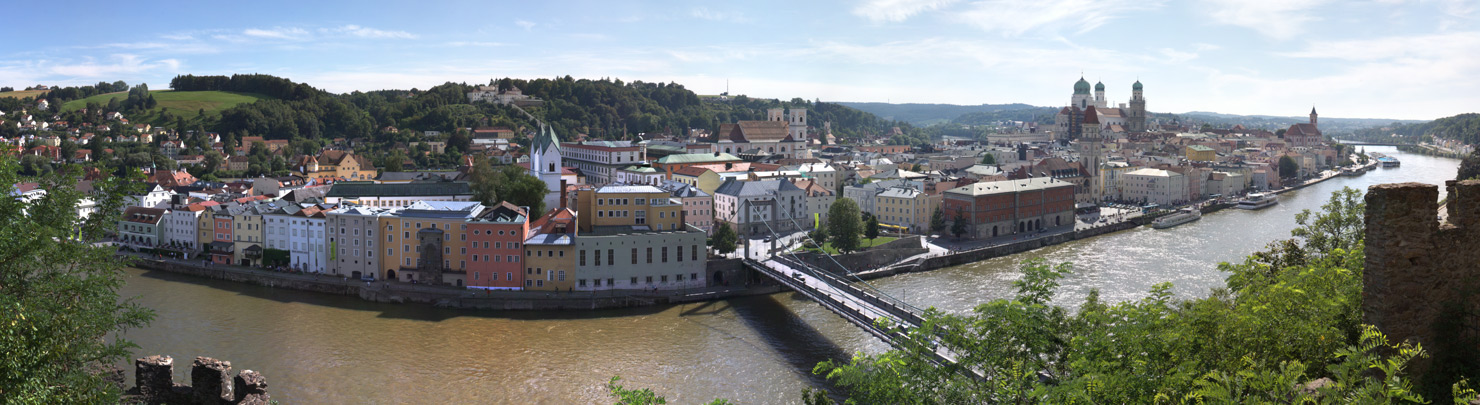
\includegraphics[width=0.97\textwidth]{../imgs/passau.jpg}
  \end{center}
  
  \begin{center}

    \vspace*{4mm}
    \Huge Teilnahmebescheinigung
    \noindent\rule{0.9\textwidth}{1pt}\\
    
    \vspace*{14mm}
        
    \Huge
    \person
    
    \vspace*{8mm}
    
    \large
    
    hat an der FOSSGIS-Konferenz 2017 in Passau teilgenommen.\\
    
    \vspace*{15mm}
    
  \end{center}


  \vspace*{18mm}

  \large
  \hskip 1cm Passau, den 24.3.2017
  
  \vspace*{12mm}
  
  \hskip 1cm FOSSGIS e.V. \hskip 1cm \includegraphics[width=5cm]{../imgs/signature.png} \hskip -6cm  \rule{7cm}{0.5pt}\\
  
  \normalsize
  \vskip -10mm \hskip 55mm Marco Lechner
  
  \newpage
} 
\end{document} 
